\pagestyle{ruled}
\begin{abstract}RMIT HIVE is endeavouring in the 2025 IREC competition, from which the avionics team is continuing its momentum in developing innovative, custom solutions that are tailor made to amateur rocketry. One such systems includes the new SOTERIA - Synchronous Operational and Telecommunications Environment for Rocket In Air - Ground station, or colloquially dubbed the GCS. This as the name implies serves as a HUB for all telecommunications operations on the ground, from which will be the first point of contact between the rocket while in flight and the avionics and by extension the RMIT IREC team on the ground. The GCS is a two part system that works off of a backplane and module based system to promote modularity and future development of successor RMIT students who wish to further develop the ground control station for additional functionality. The following report will outline all relevant documentation outlining the SOTERIA, including hardware technical information, firmware procedures, and operational bit structures for radio frequency (RF) communication. This document is designed for technically minded people whom possess a background in electrical and electronics design. If you do not possess such a background, complimentary information for clarity or background information regarding technical information will be provided. 
\end{abstract}
\section{System Overview}
\subsection{High Level System Overview}
The SOTERIA at its foundation is comprised of two PCBs and three main hardware peripherals, from which the rest of the system is built around. The most important piece of hardware that comprises the GCS is known as the PCM3365 SBC which is an embedded computer that is designed within the PC104 design constraints\cite{Advantech}. The second most important piece of hardware is custom SRAD RF modules that are meant to emulate the PC104 architecture mechanically and electronically, while the third important piece of hardware is the Raspberry Pi 5 (RPI-5), which is employed for video rendering from onboard camera modules on the rocket avionics. The integration of these individual components can be visualised as seen in figure 1.
\begin{figure}[h]
    \centering
    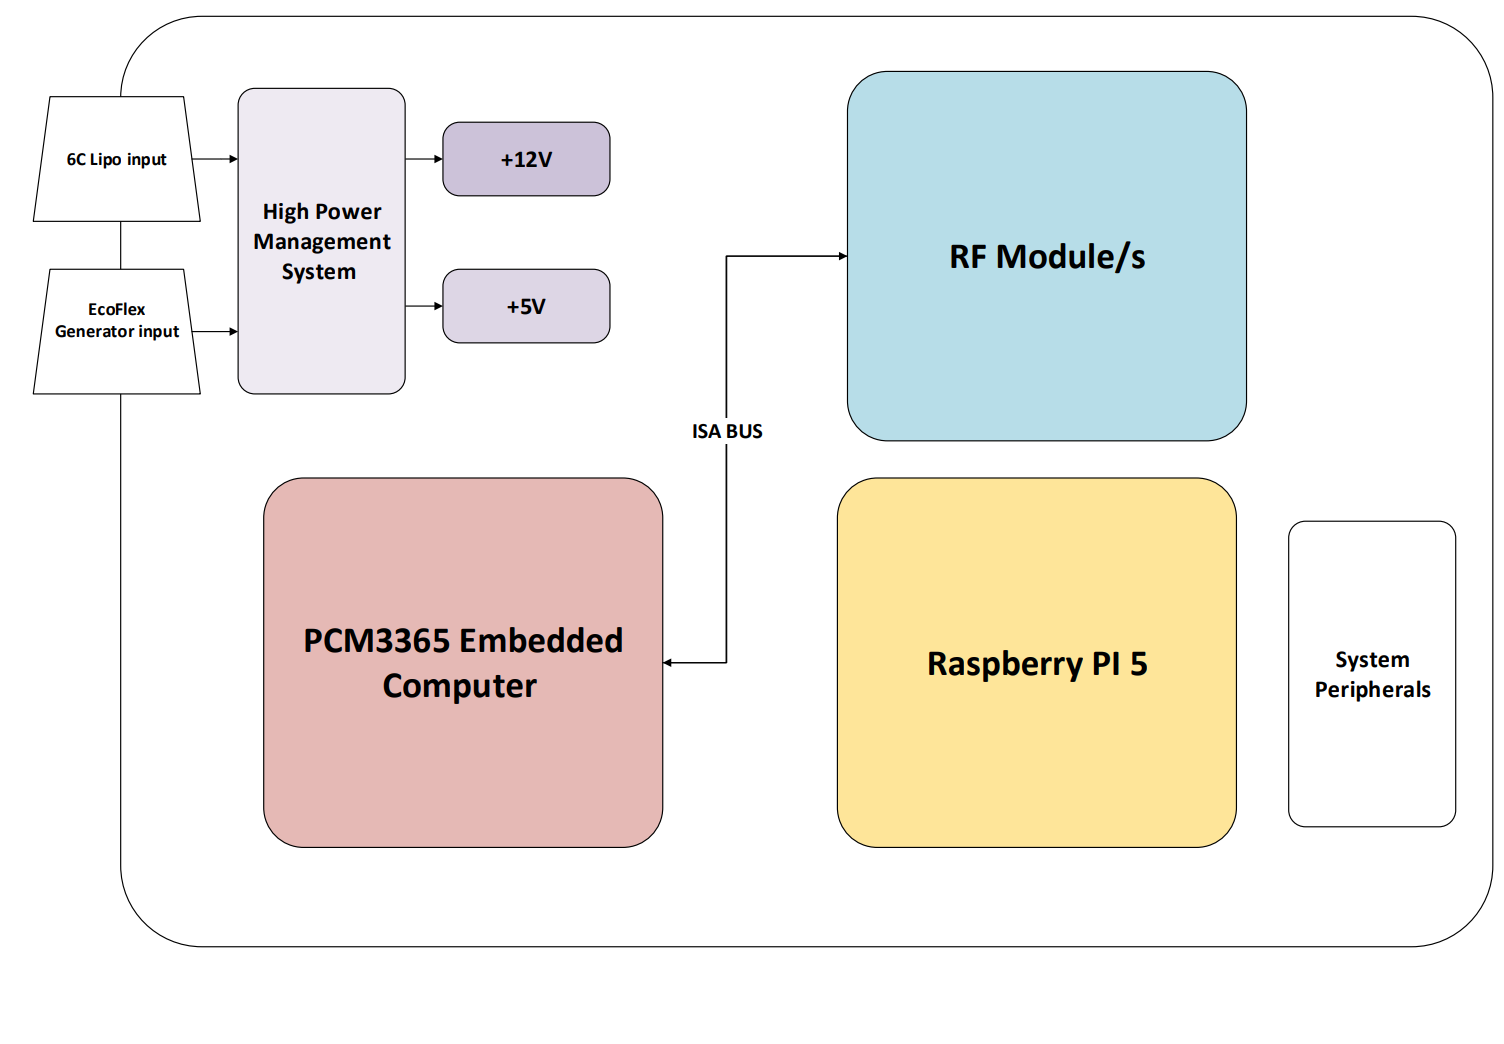
\includegraphics[scale = 0.7, ]{img/GCS simplified.PNG}
    \caption{Simplified Flowchart of entire GCS system and basic interactivity}
    \label{Figure 1: Simplified Flowchart of entire GCS system and basic interactivity}
\end{figure}
\clearpage
\subsection{High Level Requirements for the GCS}
The GCS while utilising the PCM3365, the SRAD RF modules and the RPI5 all need to interact with a numerous amount of external peripherals and protocols to ensure proper functionality of the wide system. This wider system is for peripherals such as keyboards, mouses and monitors to allow for appropriate visualisation of received telemetry, received camera feed information and outbound and inbound power and RF signals to allow for information to be sent and received from external equipment such as antennas, or external equipment such as other supporting ground equipment. The required peripherals that need to be powered by the GCS includes: 
\begin{itemize}
    \item A monitor 
    \item A Keyboard
    \item A mouse
    \item Two antenna ports
    \item Two high power inputs
    \item A DC jack output
    \item DB15 connectors for external GSE interfacing
    \item Ethernet connectivity
\end{itemize}
These surrounding peripherals require cumulatively a lot of power, and ultimately a lot of mechanical consideration to house  the necessary connectors, electrical breakout and power management to be able to successfully manage of all these peripherals continuously and concurrently. These peripherals will be covered in greater detail in future sections. 
\subsubsection{PCM3365 to RF module interfacing}
The GCS must have reliable operational capabilities between the PCM3365 which serves as the main processing HUB for the SOTERIA ground station system, whereas the the RF modules that acquire the downlinked telemetry act as slave devices that communicate to the PCM3365 primarily. The communication between these two differing devices comes down to compatibility between the available protocols the PCM3365 can offer that the onboard MCU on the RF module can accommodate. These protocols are identified through the 32 interfaceable connectors which are outlined in the PCM3365 user manual \cite{Reference_Manual}.
The PCM3365 and RF module can \textit{bidirectionally} communicate through primary communications and redundant communication methods which are defined as:
\begin{itemize}
    \item Primary communication methods
    \begin{itemize}
        \item ISA Bus
    \end{itemize}
    \item Redundant Communication Methods
      \begin{itemize}
        \item I2C
    \end{itemize}
\end{itemize}
The intricacies of how the ISA bus works specifically with respect to the PCM3365 and the firmware architecture defined by the RF modules will be defined in section 2. 
\pagebreak
\subsubsection{Raspberry Pi 5 interfacing}
The Raspberry Pi 5 will primarily be responsible for offloading heavy computational tasks that are not critical in terms of handling flight data, prelaunch states and error auxillary functionality to assist these two functionalities. Thereby, the RPI5 will not be directly interfaced during ideal operating conditions with the PCM3365 and the RF module/s, making the role of the of the RPI5 important for more graphical applications such as real-time video rendering of onboard camera systems as a subsystem of the onboard avionics, or to visualise and process a LAN based webserver that render client side information. To make this applicable for practical use, external interfacing will be available to the RPI5 through an assortment of panel mounted ethernet connectors, HDMI for a monitor, USB for peripherals, as well as a serial connector for extra interfacing with external devices. Although despite normal operation not warrenting the use of the RPI5 for critical data handling operations, redundant connectors are available for if the user wishes to employ the RPI5 as the Host computer rather than the PCM3365.
\subsubsection{Redundant RF module to RPI5 interfacing}
The RF module conveying flight telemetry to the RPI5 should only be done in the event whereby the PCM3365 is not available or is damaged, the user wishes not to use the PCM3365 or if the user is not experienced enough to use the PCM3365. In any of the previously mentioned use cases, non-ISA Bus peripherals can be employed to convey data from the RF modules to the RPI5 bypassing the ISA Bus entirely. These available options for conveying include the following:
\begin{itemize}
    \item I2C in Fast Mode
    \item USART with \textbf{no} Control Flow
\end{itemize}
Ultimately, even those these redundant options give the user options for extracting data from the RF module, it should not be employed under most use cases as to ensure preferred functionality of the GCS is upheld. 
\subsection{Radio-Frequency requirements}
With SOTERIA being a telecommunications hub, the GCS must be able to effectively receive and transmit wireless packets in the form of legally compliant RF packets. Before any development of the SOTERIA commenced, an appropriate wireless communication structure needed to be defined for the GCS whose sole purpose is to receive and transmit information to and from the rocket and surrounding support equipment. 
Much like the other avionics systems, a common technology must be selected between \textbf{ALL} equipment whether that be on the rocket or on the ground for data communication purely, such as rocket telemetry and conveying desired state and error flags to commence different operational states. As such, commonality between the following parameters must be met between all factors including the GCS:
\begin{itemize}
    \item Modulation Technique
    \item Modulation Bandwidth
    \item RF Frequency Range
\end{itemize}
Due to previous research, implementation and testing, the most suitable RF Modulation Technique has been found to be LoRa, which is  a chirp spread-spectrum modulation technique designed to operate at high range but low bandwidth. As such, all devices communicating over LoRa must furthermore share the same LoRa specific characteristics for predicable RF performance and operating range:
\begin{itemize}
    \item Output Power
    \item Coding rate
    \item Packet Size
    \item Spreading Factor
\end{itemize}
The GCS must be able to communicate to different devices on different channels within the same RF frequency range as to prevent crosstalk and interference from neighbouring or distant signals emitted by our own equipment dissimilar from the desired communication link. This means communication channels from GCS to Avionics will have it's own communication channel while the GCS to other supporting ground equipment such as the GSE will have its own channel as well. 
\break
\subsubsection{Legal Considerations of RF usage}
Due to RF communications to be unregulated or worse interfere with safety critical systems. Thereby, development of the SOTERIA ground station was heavily grounded by the laws and RF spectrum plans officiated by governing bodies such as the Australian Communications and Media Authority (ACMA)\cite{AMCA} in Australia, and the Federal Communications Commission (FCC)\cite{FCC} for the US to name a few. These regulatory bodies outline parameters that must be followed, from which breaking such laws will be treated as a criminal offense. Common factors that are often considered include:
\begin{itemize}
    \item Allowable frequency bands for general use (ISM)
    \item Allowable frequency bands permitted by licensed callsign owners
    \item Allowable output power permitted by frequency range
    \item Allowable output power by RF modulation technique
    \item The total ERP of a telecommunications system
    \item The permissible signal bandwidth as a measure of output power
    \item Field Strength emissions according to frequency range
\end{itemize}

\subsubsection{Electromechanical Integration Overview}
%outline here how the GCS will be mounted and used on launch days
\subsubsection{Subsubsection}
\subsubsection{Subsubsection}
\clearpage
\section{Technical Hardware Overview}
This section will cover more in depth technical efforts that aim to provide context to more low-level information, design rationale coupled with troubleshooting steps for potential failure modes.This section will focus on electrical and electronics hardware and will include aspects such as component selection, RF design, power management, PCB Design and DFMA consideration to ensure a manufacturable end-product. The ISA bus that is employed between the Modules and the backplane is a parallel interface that can be employed in either 8-bit or 16-bit forms. Since most onboard data often have 2 byte registers, the ISA bus has been designed to operate in 16-bit mode rather than 8 bit to reduce firmware complexity and to gain full functionality of the ISA bus. Having discussed the commonality between the backplane and the module, the below sections will go into individual detail between each subsystem. 
\subsection{GCS Module}
Having RF Module drawing inspiration behind the PC104 architecture, the module itself is 90.18mm wide and 95.88mm long, and requires at least 11mm of vertical clearance topside and bottomside for its main feature the ISA connector. The module is designed around the STM32F439IIH6 MCU which has 201 pins, of which 176 of those pins can be used for external peripheral interfacing for functions such as the ISA bus.  
Within that space it comprises the following:
\begin{itemize}
    \item A comprehensive power management system that takes supply inputs from the 5V supply from the ISA bus connector, 2S Li-ion batteries and 9V alkaline batteries.
    \item A JTAG programming interface
    \item An optional watchdog supervisor
    \item A Custom LoRa frontend
    \item Various breakout required for redundant or external device communication. 
    \item Onboard NOR storage for dedicated hardware logging of flight telemetry, state flags with time stamps and more.
\end{itemize}
Furthermore, the GCS module is designed to enable for future expansion for future flight missions, custom functionality for future development all whilst allowing for ease of integration due to its PC104 architecture. 
This was achieved by splitting the GCS module into two parts, one of which is static, and the other of which can be designed by future avionics engineers. These parts include:
\begin{itemize}
    \item ISA bus and system peripherals - STATIC - This includes:
    \begin{itemize}
        \item Level shifters for bi-directional ISA bus communication
        \item The MCU and its necessary supporting peripherals 
        \item The JTAG programming interface
        \item Circuit protection
        \item Onboard Power management
        \item Onboard Flash and peripheral breakout
        \item ISA bus Routing
    \end{itemize}
    \item User defined module functionality - DYNAMIC - This could include but not be limited to:
    \begin{itemize}
        \item RF modules for particular frequency ranges
        \item LED drivers for sequenced lighting shows
        \item Additional connectivity through acting as hub interfaces (USB).
        \item On-ground data collection.
        \item Utilised for increased Compute capabilities - employment of DSPs or FGPA.
    \end{itemize}
\end{itemize}
This gives the user to essentially create any system that can be accommodated by the ISA bus given it possesses the hardware necessary to accommodate any additional functionality, and has a communication method to the central MCU such as GPIO control pins, external interrupts or even protocols such as UART and SPI. The following sections will outline the specific technical details for each aspect of the architecture of the GCS module.
\subsubsection{MCU Design}
The chosen MCU for the GCS module was the STM32F439IIH6, which was chosen for peripheral rich interface, numerous output pins necessary for the ISA bus, its small form factor of 13mm2, and its high computational capabilities. It possesses a Arm® 32-bit Cortex®-M4 CPU with FPU, Adaptive real-time accelerator (ART Accelerator™) which allows for  0-wait state execution from Flash memory, and clock speeds up to 168Mhz maximum, and 180Mhz overclocked. 
\break
\break
The STM32F439IIH6 further boasts up to 2MB of Program flash memory organised in two banks, 256+4kB of integrated SRAM, and peripheral connectivity through either AHB or APB internal data buses. This makes the the chosen MCU a perfect blend of computational performance, cost, availability and complexity to design with, making it a desirable choice for ISA bus interpretation, and additional user defined functionality. The required pinout for the static portion of the GCS module is defined by the following figure:
\begin{figure}[h]
    \centering
    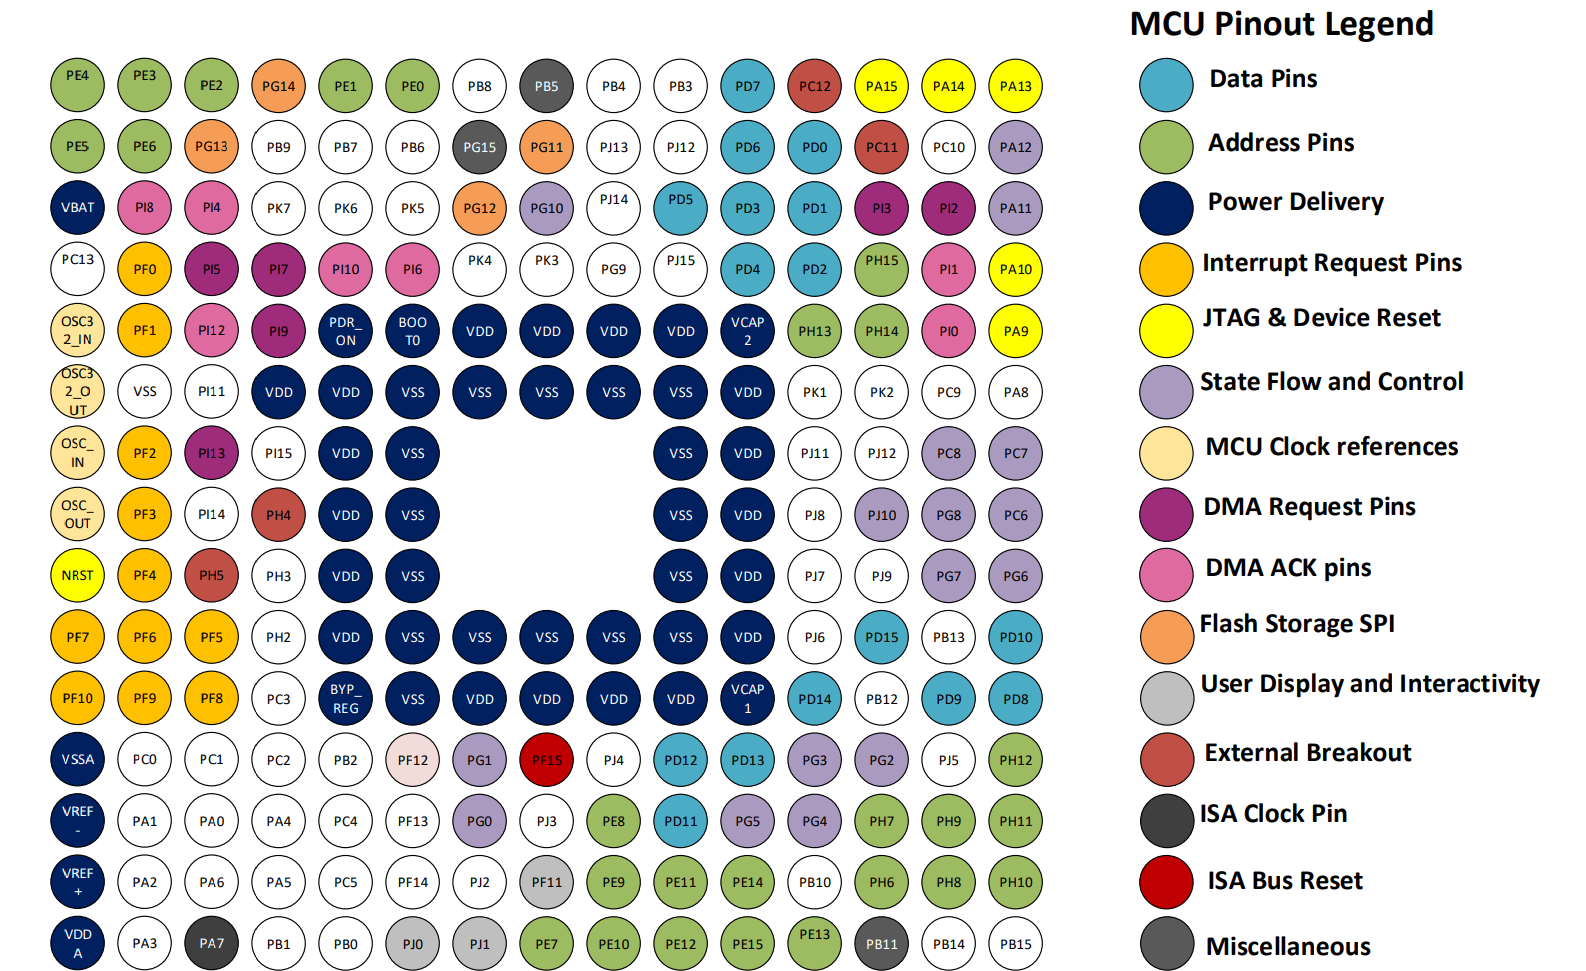
\includegraphics[width=1.1\linewidth]{img/Pinout MCU labelled.PNG}
    \caption{Caption}
    \label{fig:enter-label}
\end{figure}

\pagebreak

The interaction of how the MCU connects to every peripheral through the internal data buses can be defined through the following flow chart.
\begin{figure}[h]
    \centering
    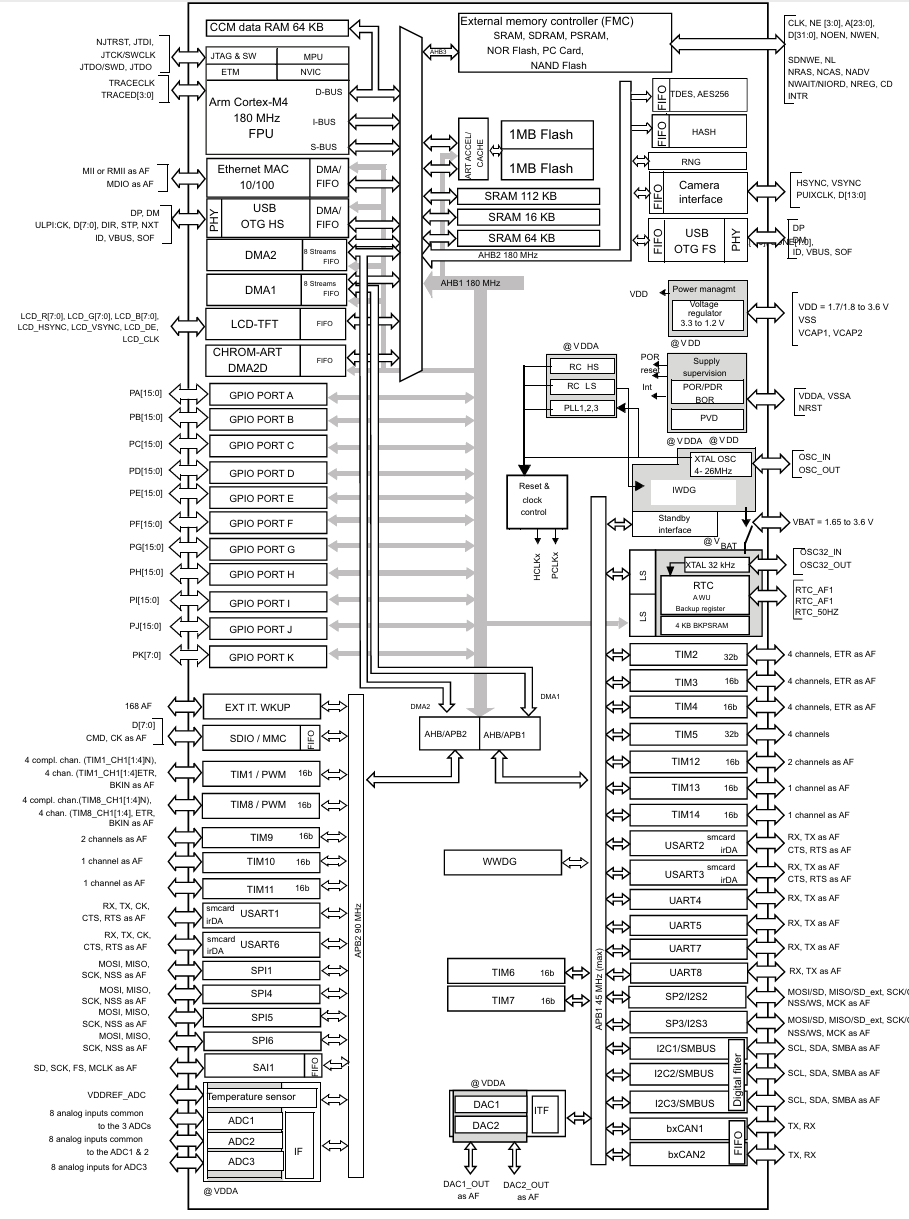
\includegraphics[width=0.9\linewidth]{img/STM32F439IIH6 Internal databus flowchart.PNG}
    \caption{Caption}
    \label{fig:enter-label}
\end{figure}
\subsubsection{ISA Bus Protocol}
\subsubsection{Power Management}
\subsubsection{Redundant Onboard Storage}
\subsection{GCS Modules - User Defined Functionality}
\subsubsection{RF Design}
\subsection{GCS Backplane}
\clearpage
\section{Firmware Architecture}
\subsection{OS level Development}


\clearpage

\section{Firmware Architecture}


\clearpage

\section{Memory and Bus Architecture}
\subsection{System Architecture}

In STM32F405xx/07xx and STM32F415xx/17xx, the main system consists of 32-bit 
multilayer AHB bus matrix that interconnects:
\begin{itemize}
    \item Eight masters:
    \begin{itemize}
        \item Cortex\textsuperscript{\textregistered}-M4 with FPU core I-bus, D-bus, and S-bus
        \item DMA1 memory bus
        \item DMA2 memory bus
        \item DMA2 peripheral bus
        \item Ethernet DMA bus
        \item USB OTG HS DMA bus
    \end{itemize}
    \item Seven slaves:
    \begin{itemize}
        \item Internal flash memory ICode bus
        \item Internal flash memory DCode bus
        \item Main internal SRAM1 (112 KB)
        \item Auxiliary internal SRAM2 (16 KB)
        \item AHB1 peripherals including AHB to APB bridges and APB peripherals
        \item AHB2 peripherals
        \item FSMC
    \end{itemize}
\end{itemize}

\noindent The bus matrix provides access from a master to a slave, enabling concurrent access and 
efficient operation even when several high-speed peripherals work simultaneously. 
The 64-Kbyte CCM (core coupled memory) data RAM is not part of the bus matrix and can be 
accessed only through the CPU. This architecture is shown in Figure 1.

\vfill{}
\begin{center}
EXAMPLE DOCUMENT \\ \small (totally not stolen from RM0090)
\end{center}
\vfill{}